% Aberdeen style guide should be followed when using this
% layout. Their template powerpoint slide is used to extract the
% Aberdeen color and logo but is otherwise ignored (it has little or
% no formatting in it anyway).
%
% http://www.abdn.ac.uk/documents/style-guide.pdf

%%%%%%%%%%%%%%%%%%%% Document Class Settings %%%%%%%%%%%%%%%%%%%%%%%%%
% Pick if you want slides, or draft slides (no animations)
%%%%%%%%%%%%%%%%%%%%%%%%%%%%%%%%%%%%%%%%%%%%%%%%%%%%%%%%%%%%%%%%%%%%%%
%Normal document mode
\documentclass[10pt,compress]{beamer}
%Draft or handout mode
%\documentclass[10pt,compress,handout]{beamer}
%\documentclass[10pt,compress,handout,ignorenonframetext]{beamer} 
%\usepackage{graphicx}
%\usepackage{epstopdf}
%\DeclareGraphicsExtensions{.gif, .ps, .eps, .png} 
%\DeclareGraphicsRule{.gif}{png}{}{`convert #1 'png:-'} 
 
%%%%%%%%%%%%%%%%%%%% General Document settings %%%%%%%%%%%%%%%%%%%%%%%
% These settings must be set for each presentation
%%%%%%%%%%%%%%%%%%%%%%%%%%%%%%%%%%%%%%%%%%%%%%%%%%%%%%%%%%%%%%%%%%%%%%

\newcommand{\shortname}{Dr Jeff Gomes}
\newcommand{\fullname}{Dr Jeff Gomes}
\institute{School of Engineering}
\newcommand{\emailaddress}{jefferson.gomes@abdn.ac.uk}
\newcommand{\logoimage}{../FigBanner/UoAHorizBanner}
\title{Renewable Energy 1: Solar and Geothermal (EG501J)}
\subtitle{Module 4: Introduction to Porous Media Fluid Flow $\&$ Heat Transfer in Geothermal Systems}
%\date[2014-15]{2014-15}
\date[]{}

%%%%%%%%%%%%%%%%%%%% Template settings %%%%%%%%%%%%%%%%%%%%%%%%%%%%%%%
% You shouldn't have to change below this line, unless you want to.
%%%%%%%%%%%%%%%%%%%%%%%%%%%%%%%%%%%%%%%%%%%%%%%%%%%%%%%%%%%%%%%%%%%%%%
\usecolortheme{whale}
\useoutertheme{infolines}

% Use the fading effect for items that are covered on the current
% slide.
\beamertemplatetransparentcovered

% We abuse the author command to place all of the slide information on
% the title page.
\author[\shortname]{%
  \fullname\\\ttfamily{\emailaddress}
}


%At the start of every section, put a slide indicating the contents of the current section.
\AtBeginSection[] {
  \begin{frame}
    \frametitle{Section Outline}
    \tableofcontents[currentsection]
  \end{frame}
}

% Allow the inclusion of movies into the Presentation! At present,
% only the Okular program is capable of playing the movies *IN* the
% presentation.
\usepackage{multimedia}
\usepackage{animate}
\usepackage{comment} 

%%%%% Color settings
\usepackage{color}
%% The background color for code listings (i.e. example programs)
\definecolor{lbcolor}{rgb}{0.9,0.9,0.9}%
\definecolor{UoARed}{rgb}{0.64706, 0.0, 0.12941}
\definecolor{UoALight}{rgb}{0.85, 0.85, 0.85}
\definecolor{UoALighter}{rgb}{0.92, 0.92, 0.92}
\setbeamercolor{structure}{fg=UoARed} % General background and higlight color
\setbeamercolor{frametitle}{bg=black} % General color
\setbeamercolor{frametitle right}{bg=black} % General color
\setbeamercolor{block body}{bg=UoALighter} % For blocks
\setbeamercolor{structure}{bg=UoALight} % For blocks
% Rounded boxes for blocks
\setbeamertemplate{blocks}[rounded]

%%%%% Font settings
% Aberdeen requires the use of Arial in slides. We can use the
% Helvetica font as its widely available like so
% \usepackage{helvet}
% \renewcommand{\familydefault}{\sfdefault}
% But beamer already uses a sans font, so we will stick with that.

% The size of the font used for the code listings.
\newcommand{\goodsize}{\fontsize{6}{7}\selectfont}

% Extra math packages, symbols and colors. If you're using Latex you
% must be using it for formatting the math!
\usepackage{amscd,amssymb} \usepackage{amsfonts}
\usepackage[mathscr]{eucal} \usepackage{mathrsfs}
\usepackage{latexsym} \usepackage{amsmath} \usepackage{bm}
\usepackage{amsthm} \usepackage{textcomp} \usepackage{eurosym}
% This package provides \cancel{a} and \cancelto{a}{b} to "cancel"
% expressions in math.
\usepackage{cancel}

\usepackage{comment} 

% Get rid of font warnings as modern LaTaX installations have scalable
% fonts
\usepackage{type1cm} 

%\usepackage{enumitem} % continuous numbering throughout enumerate commands

% For exact placement of images/text on the cover page
\usepackage[absolute]{textpos}
\setlength{\TPHorizModule}{1mm}%sets the textpos unit
\setlength{\TPVertModule}{\TPHorizModule} 

% Source code formatting package
\usepackage{listings}%
\lstset{ backgroundcolor=\color{lbcolor}, tabsize=4,
  numberstyle=\tiny, rulecolor=, language=C++, basicstyle=\goodsize,
  upquote=true, aboveskip={1.5\baselineskip}, columns=fixed,
  showstringspaces=false, extendedchars=true, breaklines=false,
  prebreak = \raisebox{0ex}[0ex][0ex]{\ensuremath{\hookleftarrow}},
  frame=single, showtabs=false, showspaces=false,
  showstringspaces=false, identifierstyle=\ttfamily,
  keywordstyle=\color[rgb]{0,0,1},
  commentstyle=\color[rgb]{0.133,0.545,0.133},
  stringstyle=\color[rgb]{0.627,0.126,0.941}}

% Allows the inclusion of other PDF's into the final PDF. Great for
% attaching tutorial sheets etc.
\usepackage{pdfpages}
\setbeamercolor{background canvas}{bg=}  

% Remove foot note horizontal rules, they occupy too much space on the slide
\renewcommand{\footnoterule}{}

% Force the driver to fix the colors on PDF's which include mixed
% colorspaces and transparency.
\pdfpageattr {/Group << /S /Transparency /I true /CS /DeviceRGB>>}

% Include a graphics, reserve space for it but
% show it on the next frame.
% Parameters:
% #1 Which slide you want it on
% #2 Previous slides
% #3 Options to \includegraphics (optional)
% #4 Name of graphic
\newcommand{\reserveandshow}[4]{%
\phantom{\includegraphics<#2|handout:0>[#3]{#4}}%
\includegraphics<#1>[#3]{#4}%
}

\newcommand{\frc}{\displaystyle\frac}
\newcommand{\red}{\textcolor{red}}
\newcommand{\blue}{\textcolor{blue}}
\newcommand{\green}{\textcolor{green}}
\newcommand{\purple}{\textcolor{purple}}
 
%% Handsout -- comment out the lines below to create handstout with 4 slides in a page with space for comments
\usepackage{handoutWithNotes}

\mode<handout>
{
\usepackage{pgf,pgfpages}

\pgfpagesdeclarelayout{2 on 1 boxed with notes}
{
\edef\pgfpageoptionheight{\the\paperheight} 
\edef\pgfpageoptionwidth{\the\paperwidth}
\edef\pgfpageoptionborder{0pt}
}
{
\setkeys{pgfpagesuselayoutoption}{landscape}
\pgfpagesphysicalpageoptions
    {%
        logical pages=4,%
        physical height=\pgfpageoptionheight,%
        physical width=\pgfpageoptionwidth,%
        last logical shipout=2%
    } 
\pgfpageslogicalpageoptions{1}
    {%
    border code=\pgfsetlinewidth{1pt}\pgfstroke,%
    scale=1,
    center=\pgfpoint{.25\pgfphysicalwidth}{.75\pgfphysicalheight}%
    }%
\pgfpageslogicalpageoptions{2}
    {%
    border code=\pgfsetlinewidth{1pt}\pgfstroke,%
    scale=1,
    center=\pgfpoint{.25\pgfphysicalwidth}{.25\pgfphysicalheight}%
    }%
\pgfpageslogicalpageoptions{3}
    {%
    border shrink=\pgfpageoptionborder,%
    resized width=.7\pgfphysicalwidth,%
    resized height=.5\pgfphysicalheight,%
    center=\pgfpoint{.75\pgfphysicalwidth}{.29\pgfphysicalheight},%
    copy from=3
    }%
\pgfpageslogicalpageoptions{4}
    {%
    border shrink=\pgfpageoptionborder,%
    resized width=.7\pgfphysicalwidth,%
    resized height=.5\pgfphysicalheight,%
    center=\pgfpoint{.75\pgfphysicalwidth}{.79\pgfphysicalheight},%
    copy from=4
    }%

\AtBeginDocument
    {
    \newbox\notesbox
    \setbox\notesbox=\vbox
        {
            \hsize=\paperwidth
            \vskip-1in\hskip-1in\vbox
            {
                \vskip1cm
                Notes\vskip1cm
                        \hrule width\paperwidth\vskip1cm
                    \hrule width\paperwidth\vskip1cm
                        \hrule width\paperwidth\vskip1cm
                    \hrule width\paperwidth\vskip1cm
                        \hrule width\paperwidth\vskip1cm
                    \hrule width\paperwidth\vskip1cm
                    \hrule width\paperwidth\vskip1cm
                    \hrule width\paperwidth\vskip1cm
                        \hrule width\paperwidth
            }
        }
        \pgfpagesshipoutlogicalpage{3}\copy\notesbox
        \pgfpagesshipoutlogicalpage{4}\copy\notesbox
    }
}
}

%\pgfpagesuselayout{2 on 1 boxed with notes}[letterpaper,border shrink=5mm]
%\pgfpagesuselayout{2 on 1 boxed with notes}[letterpaper,border shrink=5mm]
 
\begin{document}

% Title page layout
\begin{frame}
  \titlepage
  \vfill%
  \begin{center}
    \includegraphics[clip,width=0.8\textwidth]{\logoimage}
  \end{center}
\end{frame}


%%%
%%% Summary 
%%%
%\begin{frame}
%\frametitle{Overview} % Table of contents slide, comment this block out to remove it
%\tableofcontents % Throughout your presentation, if you choose to use \section{} and \subsection{} commands, these will automatically be printed on this slide as an overview of your presentation
%\end{frame}

%%%%%%%%%%%%%%%%%%%% The Presentation Proper %%%%%%%%%%%%%%%%%%%%%%%%%
% Fill below this line with \begin{frame} commands! It's best to
% always add the fragile option incase you're going to use the
% verbatim environment.
%%%%%%%%%%%%%%%%%%%%%%%%%%%%%%%%%%%%%%%%%%%%%%%%%%%%%%%%%%%%%%%%%%%%%%


%%%           %%%
%%%  SECTION  %%% 
%%%           %%%
\section{Introduction}

% SUBSECTION
 \subsection{Aims and Objectives}
%%%
%%% Slide
%%%
   \begin{frame}
     \frametitle{Aims and Objectives}
     \begin{enumerate}[(i)]
       \item <1-> XXXXXX;
 \end{enumerate}
   \end{frame}


% SECTION
 \subsection{Bibliography} 
%%%
%%% Slide
%%%
   \begin{frame}
     \frametitle{Suggested References}\scriptsize
       Literature relevant for this module:
     \begin{enumerate}[(a)]\scriptsize
       \item E. Barbier (2002) $\lq$Geothermal Energy Technology and Current Status: An Overview', Renewable $\&$ Sustainable Energy Reviews 6:3-65;
       \item H.N. Pollack, S.J. Hurter, J.R. Johnson (1993) $\lq$Heat Flow from the Earth's Interior: Analysis of the Global Data Set', Reviews of Geophysics 31:267-280;
       \item G.S. Bodvarsson, P.A. Witherspoon (1989) $\lq$Geothermal Reservoir Engineering Part 1', Geotherm. Science and Technology 2:1-68;
       \item H.K. Gupta (1980) $\lq$Geothermal Resources: An Energy Alternative', {\it In} Developments in Economic Geology 12, Chapters 3-5;
       \item K. Pruess (2002) $\lq$Mathematical Modelling of Fluid Flow and Heat Transfer in Geothermal Systems -- An Introduction in Five Lectures', United Nations University;
       \item L. Georgsson (2010) $\lq$Geophysical Methods used in Geothermal Exploration', Short Course V on Exploration for Geothermal Resources, Kenya;
       \item Documentation in \href{http://en.openei.org/wiki/Geothermal_Exploration_Best_Practices:_A_Guide_to_Resource_Data_Collection,_Analysis_and_Presentation_for_Geothermal_Projects}{OpenEI Report: Geothermal Exploration Best Practices: A Guide to Resource Data Collection, Analysis and Presentation for Geothermal Projects (2013)};
       \item Z. Chen (2006) $\lq$Computational Methods for Multiphase Flows in Porous Media', SIAM, Chapters: 1-3, 11-13;
       \item J. Finger, D. Blankenship (2010) $\lq$Handbook of Best Practices for Geothermal Drilling', Sandia National Laboratories Report, \href{http://www1.eere.energy.gov/geothermal/pdfs/drillinghandbook.pdf}{SAND2010-6048}.
     \end{enumerate}
\end{frame}


%%%           %%%
%%%  SECTION  %%% 
%%%           %%%
 \section{Geothermal Energy Science}

%%% SUBSECTION
\subsection{Natural Geothermal Gradients}

%%%
%%% Slide
%%%
\begin{frame}
 \frametitle{Fourier's Law: Thermal Conduction}
  \begin{columns}
   \begin{column}[c]{0.45\linewidth}
    \begin{enumerate}[1.] \scriptsize
       \item <1-> \blue{Gradient} is a vector operator (symbol: $\nabla$) used to represent the slope of function with respect to a variable, i.e., 
          \begin{displaymath}
             \nabla \phi \left(x, y, z\right) = \left( \frc{\partial \phi}{\partial x}, \frc{\partial \phi}{\partial y}, \frc{\partial \phi}{\partial z}\right)
          \end{displaymath} 
       \item <2-> Temperature rises approximately 2.5$^{\circ}$C at every 100 meters (we may consider negligible oscillations in radial and axial directions),
          \begin{eqnarray}
             \nabla T  &=& \frc{\partial T}{\partial x} = \frc{\Delta T}{\Delta x} \approx \frc{2.5}{100} \frc{^{\circ}\text{C}}{m}  \nonumber \\
                       &=& 0.025 \frc{^{\circ}\text{C}}{m} = 0.025 \frc{K}{m} \nonumber
          \end{eqnarray} 
       \item <3-> This means that to reach \blue{125$^{\circ}$C}, we would need to drill wells at a \blue{depth of 5 km}
       \item <4-> Geothermal gradients can be enhanced through special geologic conditions, e.g., regions where molten rock has raised to shallower depths or;
       \item <4-> In regions with \blue{deep fluid circulation}.
    \end{enumerate}
   \end{column}
   \begin{column}[c]{0.55\linewidth}
     \vbox{
        \hbox{\hspace{1cm}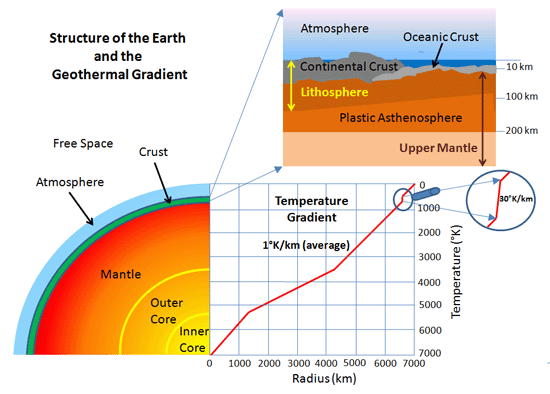
\includegraphics[width=5.cm,clip]{./Pics/geothermal_gradient.png}}
        \hbox{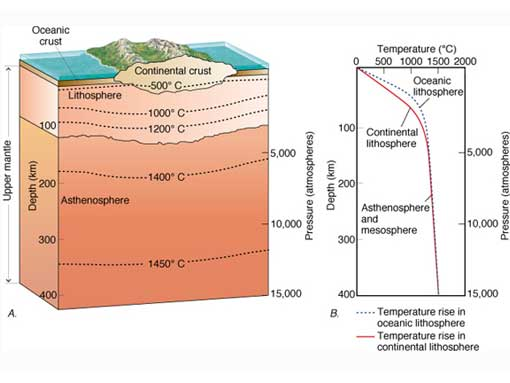
\includegraphics[width=3.5cm,clip]{./Pics/geothermalgradient.jpg}
              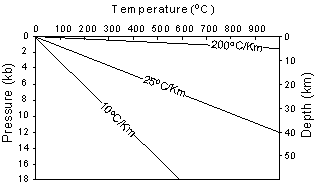
\includegraphics[width=3.3cm,clip]{./Pics/geotherms.png}}
     }
   \end{column}  
  \end{columns}
\end{frame}

%%%
%%% Slide
%%%
\begin{frame}
 \frametitle{Fourier's Law: Thermal Conduction}
  \begin{columns}
    \begin{column}[c]{0.45\linewidth}
      \begin{enumerate}[1.]\setcounter{enumi}{5} \scriptsize
        \item <1-> The fundamental law of {\it heat conduction} states that heat flows in a \underline{continuous} rock due to temperature differences throughout the medium;
        \item <2-> The transfer of energy occurs from zones of higher temperature to zones of lower temperature ({\it Zeroth Law of Thermodynamics});
        \item <3-> The Fourier's law states that the energy flow (i.e., heat flux, $q$) is proportional to the temperature gradient, $q\propto \nabla T$,
           \visible<3->{\begin{equation}
              q = - \kappa\nabla T
           \end{equation}
           where $\kappa$ is the constant of proportionality and is called \blue{thermal conductivity coefficient};}
        \item <4-> $\kappa \left[\text{in }W.\left(m.K\right)^{-1}\right]$ is a parameter obtained experimentally that may vary in space, i.e., $\kappa = \kappa\left(x, y, z\right)$ and is also a function of temperature -- $\kappa = \kappa\left(x, y, z, T\right)$;
        \item <5-> For an averaged rock thermal conductivity, $\kappa_{\text{rock}}\approx 2.0\;\frc{W}{m.K}\rightarrow q=-0.05\frc{W}{m^{2}}$;
        \item <6-> Thus over an area of 1 km$^{2}$, the crustal \blue{heat flow rate} would be of \blue{50 kW};
      \end{enumerate}
    \end{column}
    \begin{column}[c]{0.55\linewidth}
          \href{http://www.springer.com/cda/content/document/cda_downloaddocument/9783642340222-c2.pdf?SGWID=0-0-45-1456221-p174676272}{\hspace{-1.cm}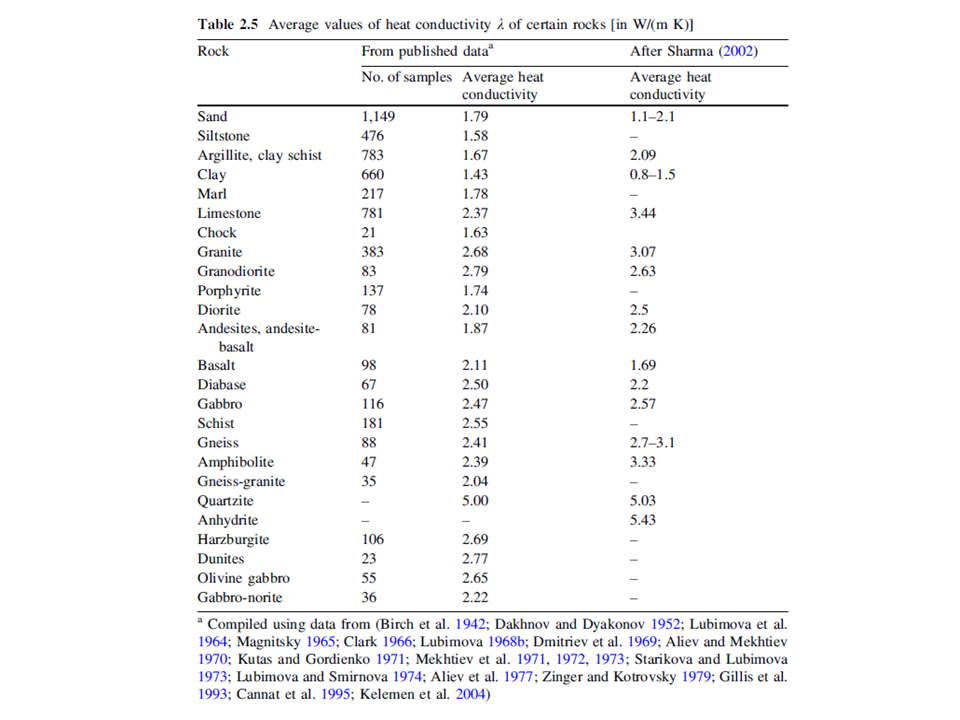
\includegraphics[width=1.2\columnwidth]{./Pics/ListRocksConductivity.png}\\
          \scriptsize From L. Eppelbaum, I. Kutasov, A. Pilchin, Applied Geothermics, Chapter 2.}
    \end{column}  
  \end{columns}
\end{frame} 

%%%
%%% Slide
%%%
\begin{frame}
 \frametitle{Fourier's Law: Thermal Conduction}
    \begin{enumerate}[1.]\setcounter{enumi}{11} \scriptsize
       \item <1-> This is very \underline{small} if compared with common \blue{heat extraction rates} in geothermal fields of \red{10-10$^{2}$ MW};
       \item <2-> Therefore \underline{\blue{Thermal Conduction}} is \red{not the only} heat transfer mechanism.
    \end{enumerate}

    \visible<3->{\begin{center}
       \href{http://www.gly.uga.edu/railsback/PGSG/PGSGmain.html}{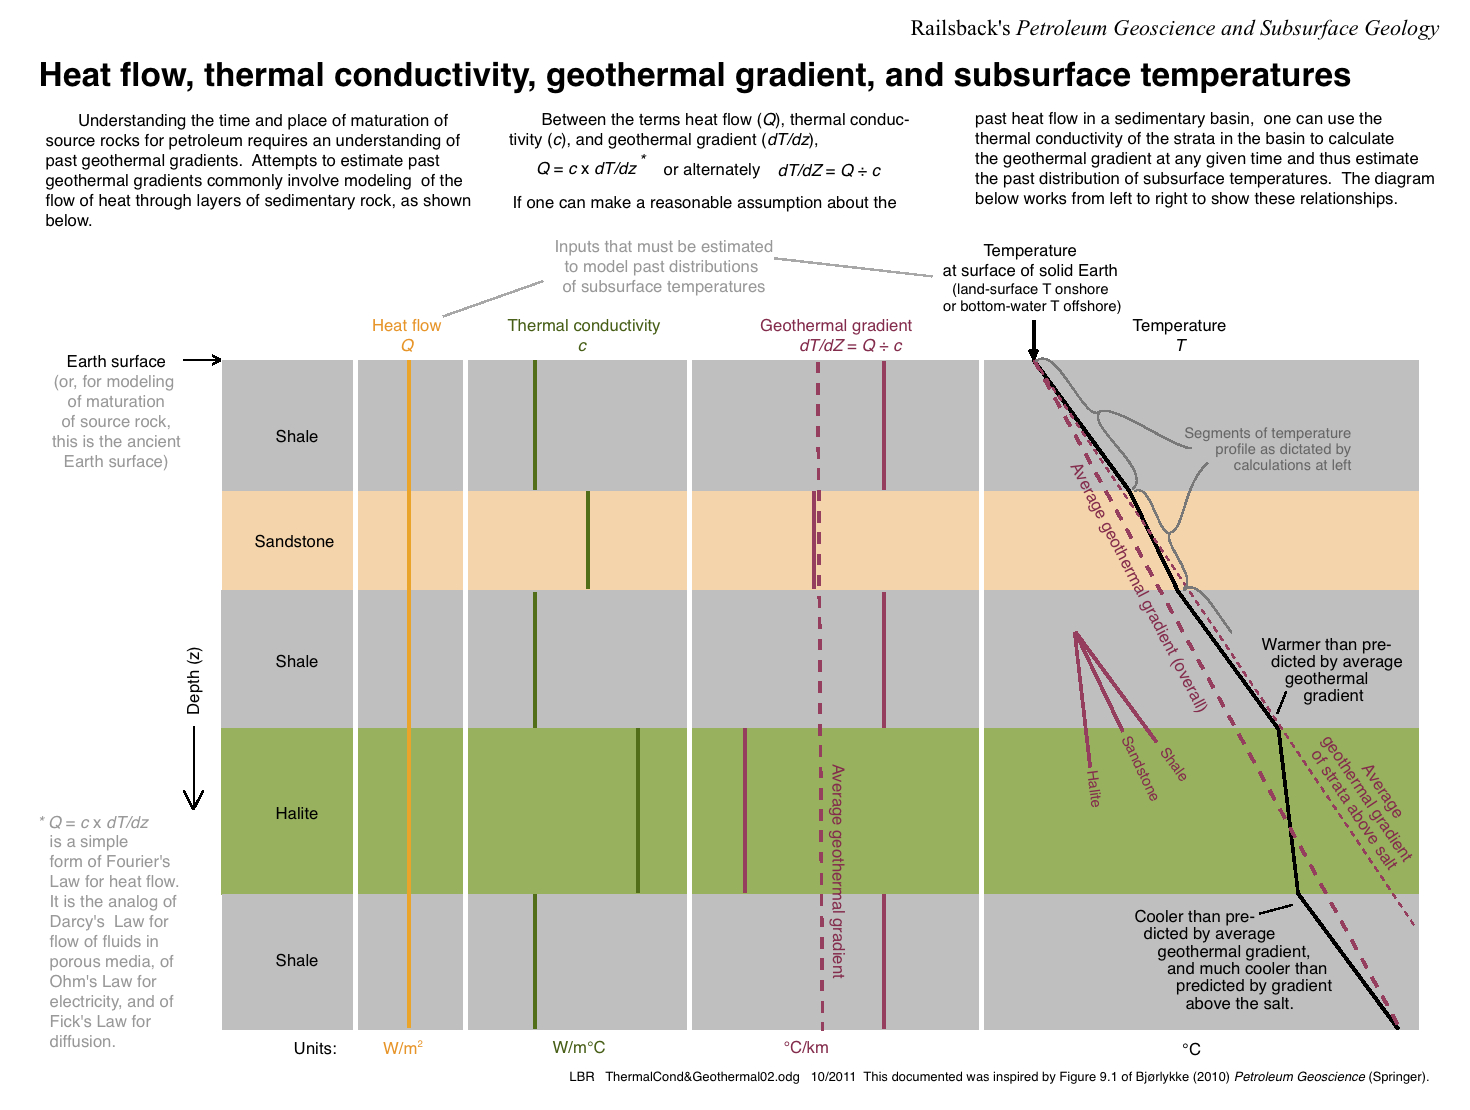
\includegraphics[width=8.cm, height=6.5cm,clip]{./Pics/ThermalCond_Geothermal02.jpg}\\
             \scriptsize From L.B. Railsback (Georgia, USA), Petroleum Geoscience and Subsurface Geology.}
    \end{center}}
\end{frame}


%%%
%%% SUBSECTION
%%%
\subsection{Hydrothermal Convection Systems}

%%%
%%% Slide
%%%
\begin{frame}
 \frametitle{Thermal Convection}
    \begin{enumerate}[1.] \scriptsize
       \item <1-> Let's consider a reservoir containing a geothermal fluid of density $\rho$; 
       \item <2-> Under static conditions (i.e., no flow), the pressure is expressed as the weight of the fluid column per unit area, and increases with depth $z$ as,
            \visible<2->{\begin{equation}
                \int\limits_{P_{0}}^{P}dP = \int\limits_{z_{0}}^{z}\rho g dz \Longrightarrow \blue{P(z) = P_{0} + \rho g z},
            \end{equation} 
            where $g$ is the gravity acceleration. Here we assume that pressure does not change in axial and radial directions;}
       \item <3-> Densities of geothermal fluids can be expressed as functions of temperature, pressure (and therefore depth) and salinity $\left(\mathcal{C}_{S}\right)$, i.e., $\rho=\rho\left(T,P,\mathcal{C}_{S}\right)$
       \item <4-> Algebraic expressions that correlate pressure, temperature and specific volume (PvT) are commonly called \underline{\it Equations of State} (EOS);
       \item <5-> An example of EOS that represents the impact of pressure, temperature in the fluid density is, 
            \visible<5->{\begin{equation}
                \rho = \rho_{0}\left[1 - \alpha\left(T-T_{0}\right)+\beta\left(P-P_{0}\right)\right]
            \end{equation}
            where $\alpha$ and $\beta$ are the expansivity and compressibility coefficients, respectively;}
    \end{enumerate}
\end{frame}


%%%
%%% Slide
%%%
\begin{frame}
 \frametitle{Thermal Convection}
  \begin{columns}
   \begin{column}[c]{0.45\linewidth}
    \begin{enumerate}[1.]\setcounter{enumi}{5} \scriptsize
       \item <1-> As warmer fluid (e.g., brine) is less dense than cold fluid $\Longrightarrow$ column of warmer fluid weights less than the cold fluid column;
       \item <2-> \red{Thermal Buoyancy} is a physical phenomena in which cold $\&$ denser fluid displace warmer $\&$ lighter fluid;
       \item <3-> This can be extended to geothermal sources, if we assume that the cold and denser water is the \underline{discharge fluid}, {\it whereas} denser warmer $\&$ lighter fluid represents the conditions in the centre of the field; 
       \item <4-> For \blue{hydrothermal circulation} to occur, we only need a \blue{temperature gradient}. 
    \end{enumerate}
   \end{column}
   \begin{column}[c]{0.55\linewidth}
     \begin{center}
        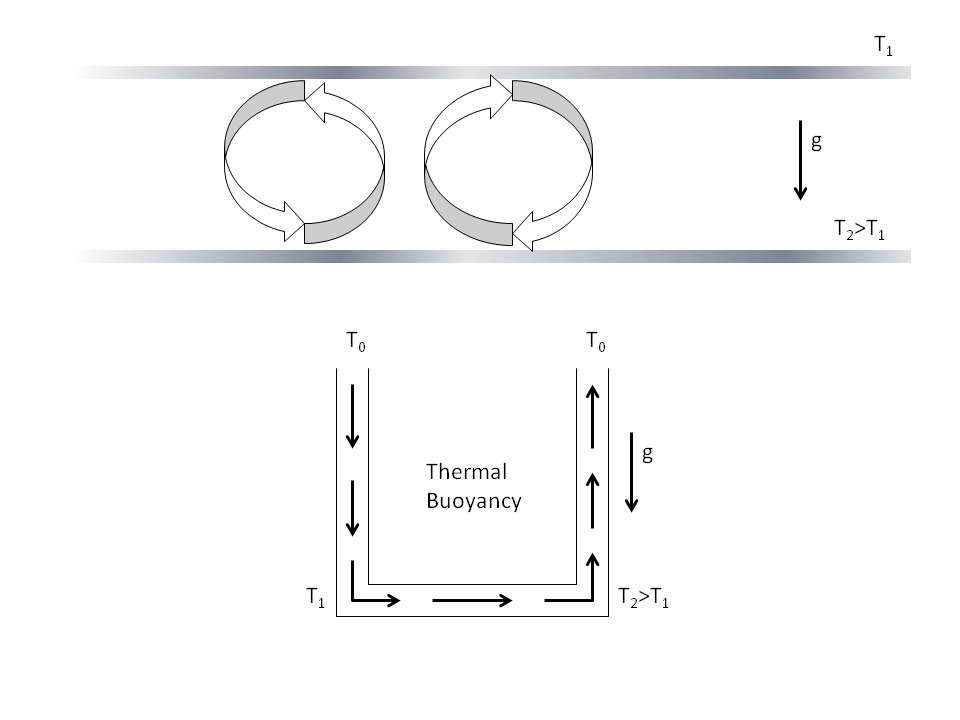
\includegraphics[width=\columnwidth,clip]{./Pics/GeothermalConvection.png}
     \end{center}
   \end{column}  
  \end{columns}
\end{frame}



%%%
%%% SUBSECTION
%%%
\subsection{Porous Media Flow}

%%%
%%% Slide
%%%
\begin{frame}
 \frametitle{Geothermal Darcy Flows}
  \begin{columns}
   \begin{column}[c]{0.45\linewidth}
    \begin{enumerate}[1.] \scriptsize
       \item <1-> Fluid motion is due to forces, in particular pressure and gravity forces;
       \item <2-> Henry Darcy (1986) established the correlation between fluid flow and forces based on experiments of water flowing through a sandpack;
       \item <3-> The rate of fluid flow depends on \blue{pressure gradient, $\nabla P$},
          \visible<3->{\begin{equation}
             \dot{Q} = - \mathcal{K} \frc{\rho}{\mu}\nabla P
          \end{equation}
          where $\dot{Q}$ is the mass flow rate per cross-sectional area, $\mu$ is the fluid viscosity. $\mathcal{K}$ is the absolute permeability;}
       \item <4-> In 3D, this equation can be expressed as, 
          \begin{displaymath}
            \begin{pmatrix} \dot{Q_{x}}\\ \\\dot{Q_{y}}\\ \\\dot{Q_{z}}\end{pmatrix} = - \mathcal{K} \frc{\rho}{\mu} \begin{pmatrix} \frc{\Delta P}{\Delta x} \\ \\\frc{\Delta P}{\Delta y} \\ \\\frc{\Delta P}{\Delta z}-\rho g \end{pmatrix};
          \end{displaymath}
    \end{enumerate}
   \end{column}
   \begin{column}[c]{0.55\linewidth}
    \begin{enumerate}[1.]\setcounter{enumi}{9} \scriptsize
       \item <5-> Or in matricial form,
          \visible<3->{\begin{equation}
            \underline{\dot{Q}} = - \mathcal{K} \frc{\rho}{\mu} \left(\nabla P - \rho \underline{g}\right),\label{eqn:preDarcy}
          \end{equation}
          with $\underline{g} = \left( 0\;\;\; 0\;\;\; g \right)^{T}$.}
    \end{enumerate}
     \begin{center}
        \visible<3->{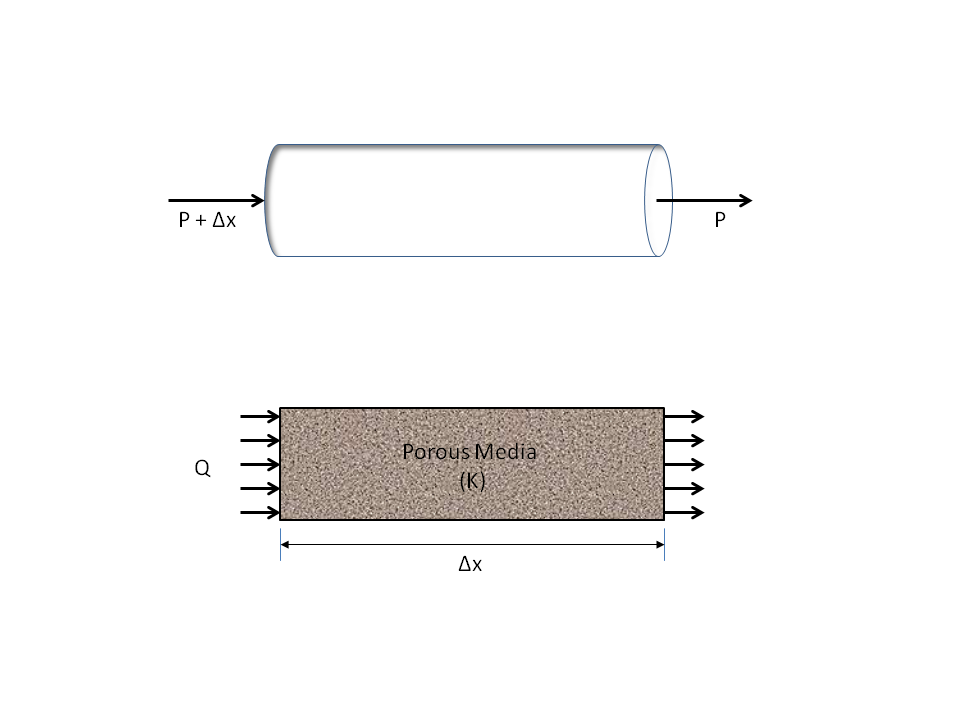
\includegraphics[width=1.1\columnwidth,clip]{./Pics/Geothermal_PorousMediaFlow.png}}
     \end{center}
   \end{column}  
  \end{columns}
\end{frame}



%%%
%%% Slide
%%%
\begin{frame}
 \frametitle{Geothermal Darcy Flows}
   \begin{columns}
      \begin{column}[c]{0.5\linewidth}
         \begin{enumerate}[1.]\setcounter{enumi}{10} \scriptsize
            \item <1-> Dividing Eqn.~\ref{eqn:preDarcy} by $\rho$ leads to the volumetric flux, $\underline{u}$,
               \visible<1->{\begin{equation}
                  \frc{\underline{\dot{Q}}}{\rho} = \red{\underline{u} = - \frc{\mathcal{K}}{\mu}\left(\nabla P - \rho \underline{g}\right)},\label{eqn:Darcy}
               \end{equation}
               where $\underline{u}$ is often referred as \blue{\it Darcy velocity};}
            \item <2-> However this is not really the velocity in which the fluid flows -- which is called \blue{\it pore velocity}, \blue{$\underline{v}$}; 
            \item <3-> $\underline{u}$ and $\underline{v}$ are related by the following relationship,
               \visible<3->{\begin{displaymath}
                  \underline{u} = \phi \underline{v}
               \end{displaymath} 
               where $\phi$ is the rock porosity.}
            \item <4-> Before we continue, we need to establish a few very important definitions:
               \begin{enumerate}[(a)]\scriptsize
                  \item <4-> \blue{(Absolute) Porosity $\left(\phi\right)$} is the ratio between total volume of voidage in the rock pore and the volume of the rock,
                     \begin{equation}
                        \phi = \frc{V_{\text{void}}}{V_{\text{total}}};
                     \end{equation}
                  \item <5-> \blue{Saturation $\left(S\right)$} is a variable relevant \underline{only} when \underline{more than one} fluid (or phase) is present
               \end{enumerate}
         \end{enumerate}  
      \end{column}
      \begin{column}[c]{0.5\linewidth}
         %\begin{enumerate}[(a)]\setcounter{enumi}{1} \scriptsize
             %\item <5-> 
           \visible<5->{\scriptsize (multiphase systems). Saturation can be  defined as the volume fraction of the occupied pores by fluids,  
                     \begin{equation}
                        S_{\alpha} = \frc{V_{\alpha}}{V_{\text{void}}}
                     \end{equation}}
         %\end{enumerate}  
         \begin{figure}%
            \vspace{-.5cm}
            \vbox{
                  \visible<4->{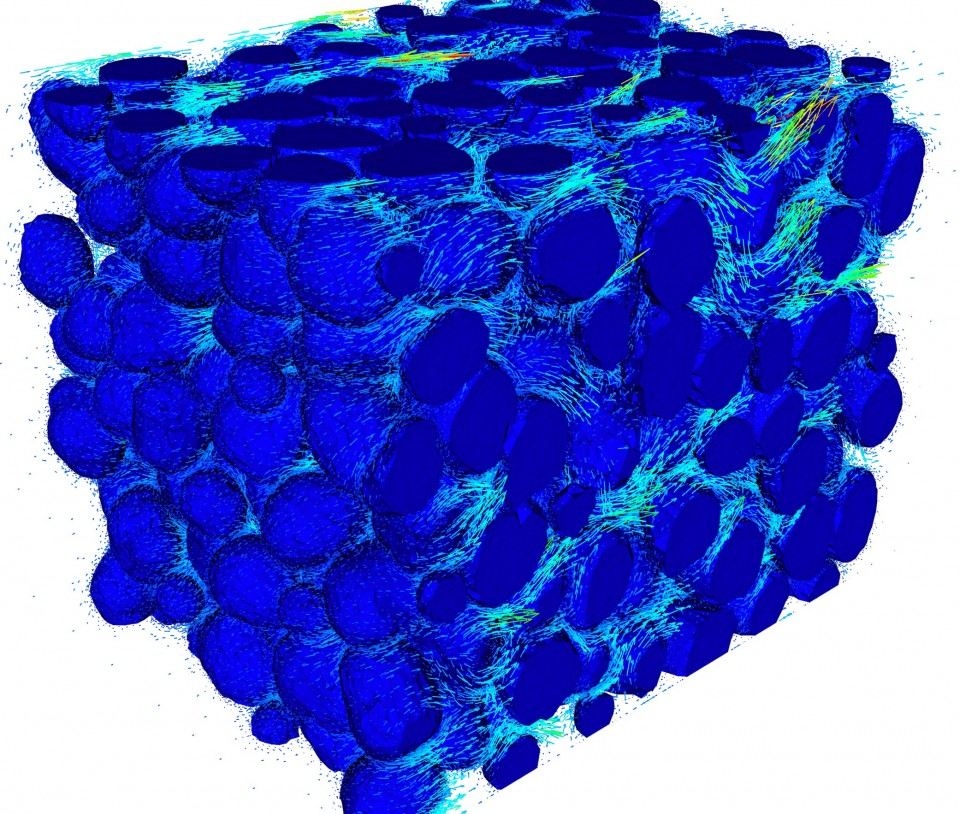
\includegraphics[width=3.cm,clip]{./Pics/two-phase-method-flow-in-grain-pack-e1262722458668.jpg}}
                  \visible<5->{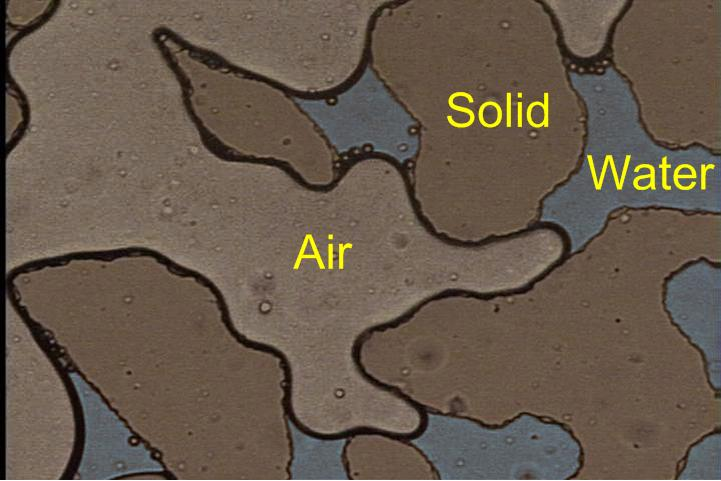
\includegraphics[width=3.cm,clip]{./Pics/Unsat1.jpg}}
            }
         \end{figure}
      \end{column}
   \end{columns}
\end{frame}









%%%%%%%%%%%%%%%%%%%%%%%%%%%%%%%%%%%%%%%%%%%%%%%%%%%%%%%%%%%%%%%%%%%%%%%%%
%%%%%%%%%%%%%%%%%%%%%%%%%%%%%%%%%%%%%%%%%%%%%%%%%%%%%%%%%%%%%%%%%%%%%%%%%
%%%%%%%%%%%%%%%%%%%%%%%%%%%%%%%%%%%%%%%%%%%%%%%%%%%%%%%%%%%%%%%%%%%%%%%%%


%%%           %%%
%%%  SECTION  %%% 
%%%           %%%
 \section{Geothermal Project Development} % From IFC-IGA_Geothermal_Exploration_Best_Practices-March2013

%%%
%%% Slide
%%%
\begin{frame}
 \frametitle{Phases for Geothermal Project Developments} 
    There is usually 7 phases for any \blue{geothermal} (or subsurface) \blue{project development}: 
    \begin{enumerate}[1.]
       \item <1-> \blue{Preliminary Survey;}
       \item <1-> Exploration; 
       \item <1-> Test Drilling;
       \item <1-> Project Review and Planning;
       \item <1-> Field Development; 
       \item <1-> Power Plant Construction;
       \item <1-> Commissioning and Operation;
    \end{enumerate}
\end{frame}

%%%
%%% Slide
%%%
\begin{frame}
 \frametitle{Phases for Geothermal Project Developments: \\1. Preliminary Survey} 

    Initial assessment (nationally and/or internationally) of the available information on:
    \begin{enumerate}[{1.}1]
       \item <1-> Finances, Economics and Legal issues:
          \begin{enumerate}[(a)]
             \item<2-> Power (electricity) market (and/or power purchase agreements, PPA, and/or feed in tariff);
             \item<2-> Resources ownership (i.e., land/water right, mining laws etc);
             \item<2-> Institutional and regulatory framework;
          \end{enumerate}
       \item <3-> Environmental regulations; 
       \item <4-> Infrastructure (e.g., roads, water, communication, electrical transmission).
    \end{enumerate}
\end{frame}

%%%
%%% Slide
%%%
\begin{frame}
 \frametitle{Phases for Geothermal Project Developments} 
    \begin{enumerate}[1.]
       \item <1-> Preliminary Survey;
       \item <2-> \blue{Exploration}; 
       \item <1-> Test Drilling;
       \item <1-> Project Review and Planning;
       \item <1-> Field Development; 
       \item <1-> Power Plant Construction;
       \item <1-> Commissioning and Operation;
    \end{enumerate}
\end{frame}

%%%
%%% Slide
%%%
\begin{frame}
 \frametitle{Phases for Geothermal Project Developments: \\ 2. Exploration} 

    \begin{enumerate}[{2.}1]\scriptsize
       \item <1-> The \blue{exploration phase} aims to minimise risks related to resource temperature, depth, productivity and sustainability before drilling assessment;
       \item <2-> \blue{Exploration} usually starts by collecting data from existing surrounding surface, subsurface and wells sensors through geological. geochemical and geophysical methods.
       \item <3-> Usual \blue{exploration} surveys include:
          \begin{enumerate}[(a)]\scriptsize
             \item<4-> Geochemical assessment
                \begin{enumerate}[i)]\scriptsize
                   \item<4-> Geothermometry;
                   \item<4-> Electrical conductivity;
                   \item<4-> pH;
                   \item<4-> Fluid flow rate;
                   \item<4-> Soil morphology.
                \end{enumerate}
             \item<5-> Geophysical assessment
                \begin{enumerate}[i)]\scriptsize
                   \item<5-> Gravity;
                   \item<5-> Electrical resistivity;
                   \item<5-> Temperature gradient drilling;
                   \item<5-> 2D and 3D seismics.
                \end{enumerate}
             \item<6-> Surface assessment
                \begin{enumerate}[i)]\scriptsize
                   \item<6-> Surface geology;
                   \item<6-> Geothermal surface features.
                \end{enumerate}
             \item<7-> etc.
          \end{enumerate}
       \item <8-> With this info, models (conceptual and numerical) are built to support the \blue{pre-feasibility study}. 
    \end{enumerate}
\end{frame}
 

%%%
%%% Slide
%%%
\begin{frame}
 \frametitle{Phases for Geothermal Project Developments} 
    \begin{enumerate}[1.]
       \item <1-> Preliminary Survey;
       \item <1-> Exploration; 
       \item <2-> \blue{Test Drilling};
       \item <1-> Project Review and Planning;
       \item <1-> Field Development; 
       \item <1-> Power Plant Construction;
       \item <1-> Commissioning and Operation;
    \end{enumerate}
\end{frame}


%%%
%%% Slide
%%%
\begin{frame}
 \frametitle{Phases for Geothermal Project Developments: \\ 3. Test Drilling}
  \begin{columns}
    \begin{column}[l]{0.45\linewidth}     
       \begin{enumerate}[{3.}1]\scriptsize
          \item <1-> Usually 2-3 wells are drilled to demonstrate the commercial feasibility of production and injection;
          \item <2-> Drilling, logging and testing will improve the understanding of the subsurface resources enabling,  
          \begin{enumerate}[(a)]\scriptsize
             \item<3-> Further estimate of heat resource;
             \item<4-> Determination of the average well productivity;
             \item<5-> Selection of the wells sites, targets, well path and design for the remaining production and injection wells;
             \item<6-> Development of a \blue{preliminary design for the power plant}.
          \end{enumerate}
       \end{enumerate}
       %\begin{center}
           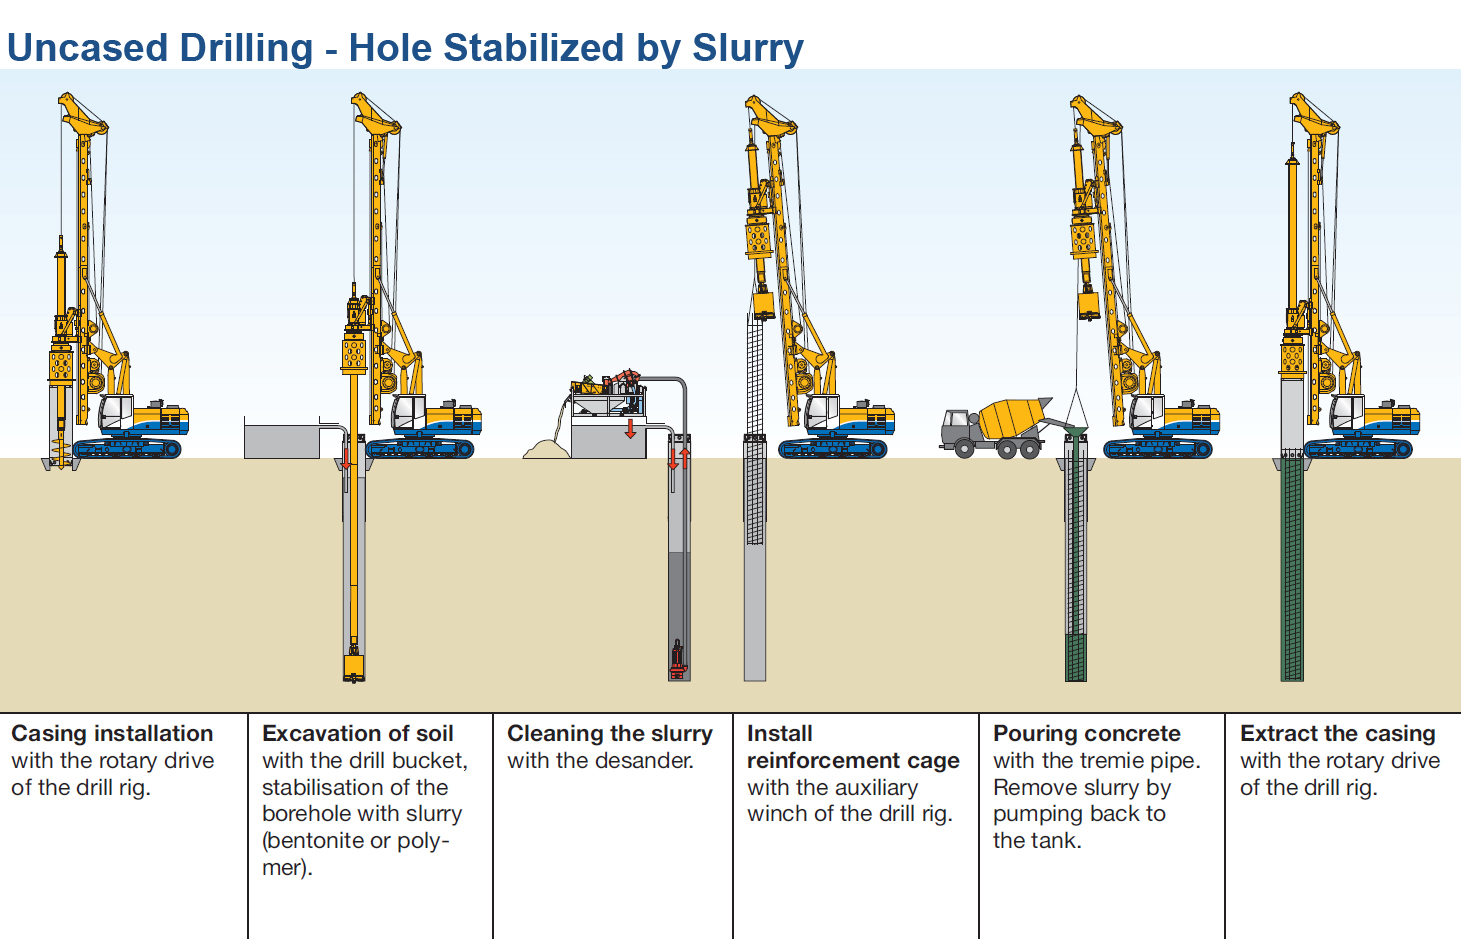
\includegraphics[width=5.6cm,height=2.7cm,clip]{./Pics/Uncased-Drilling-1.jpg}
       %\end{center}
    \end{column}
    \begin{column}[l]{0.55\linewidth} 
       \vbox{
          \hbox{
             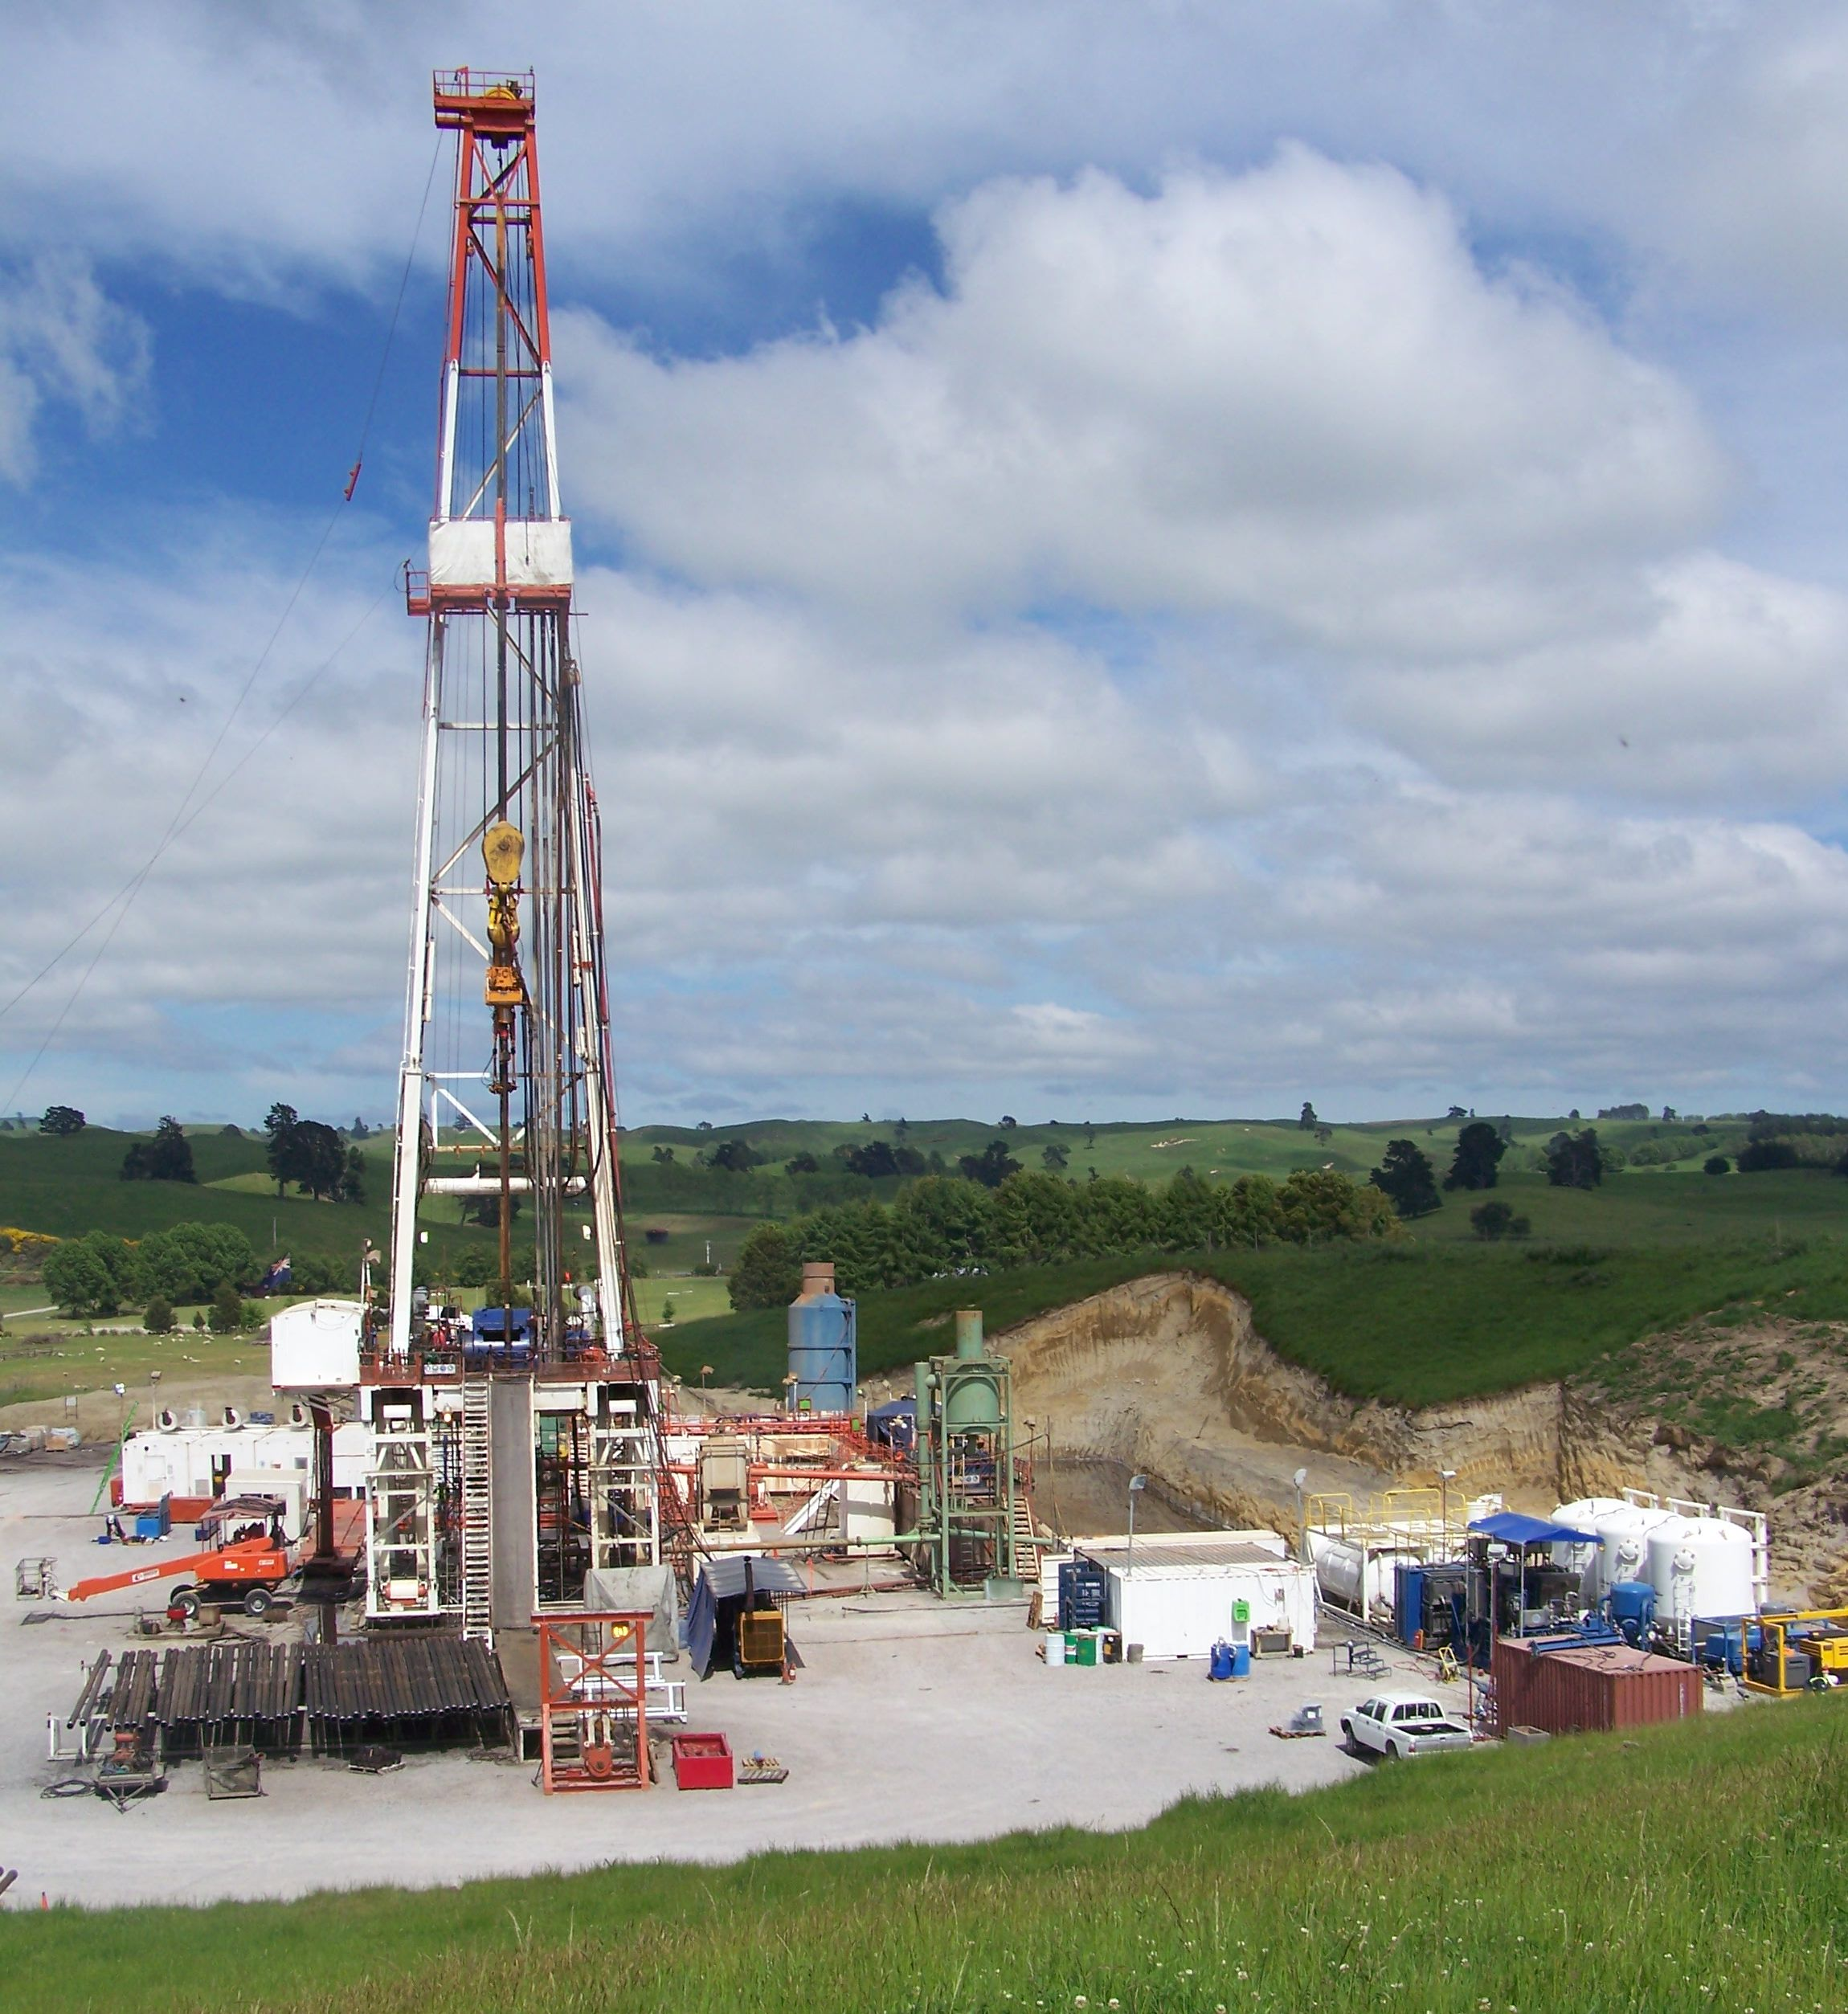
\includegraphics[width=0.5\columnwidth,clip]{./Pics/Geothermal_drilling_at_Te_Mihi_NZ.jpg}
             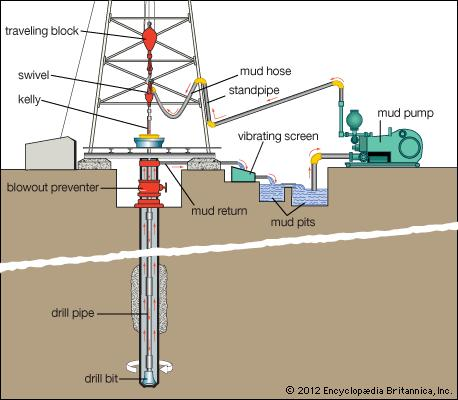
\includegraphics[width=0.5\columnwidth,clip]{./Pics/Drilling.jpg}
          }
          \hbox{
             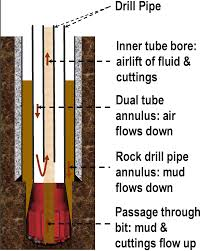
\includegraphics[width=0.35\columnwidth,clip]{./Pics/DTRC_Diagram.jpg}\hspace{.53cm}
             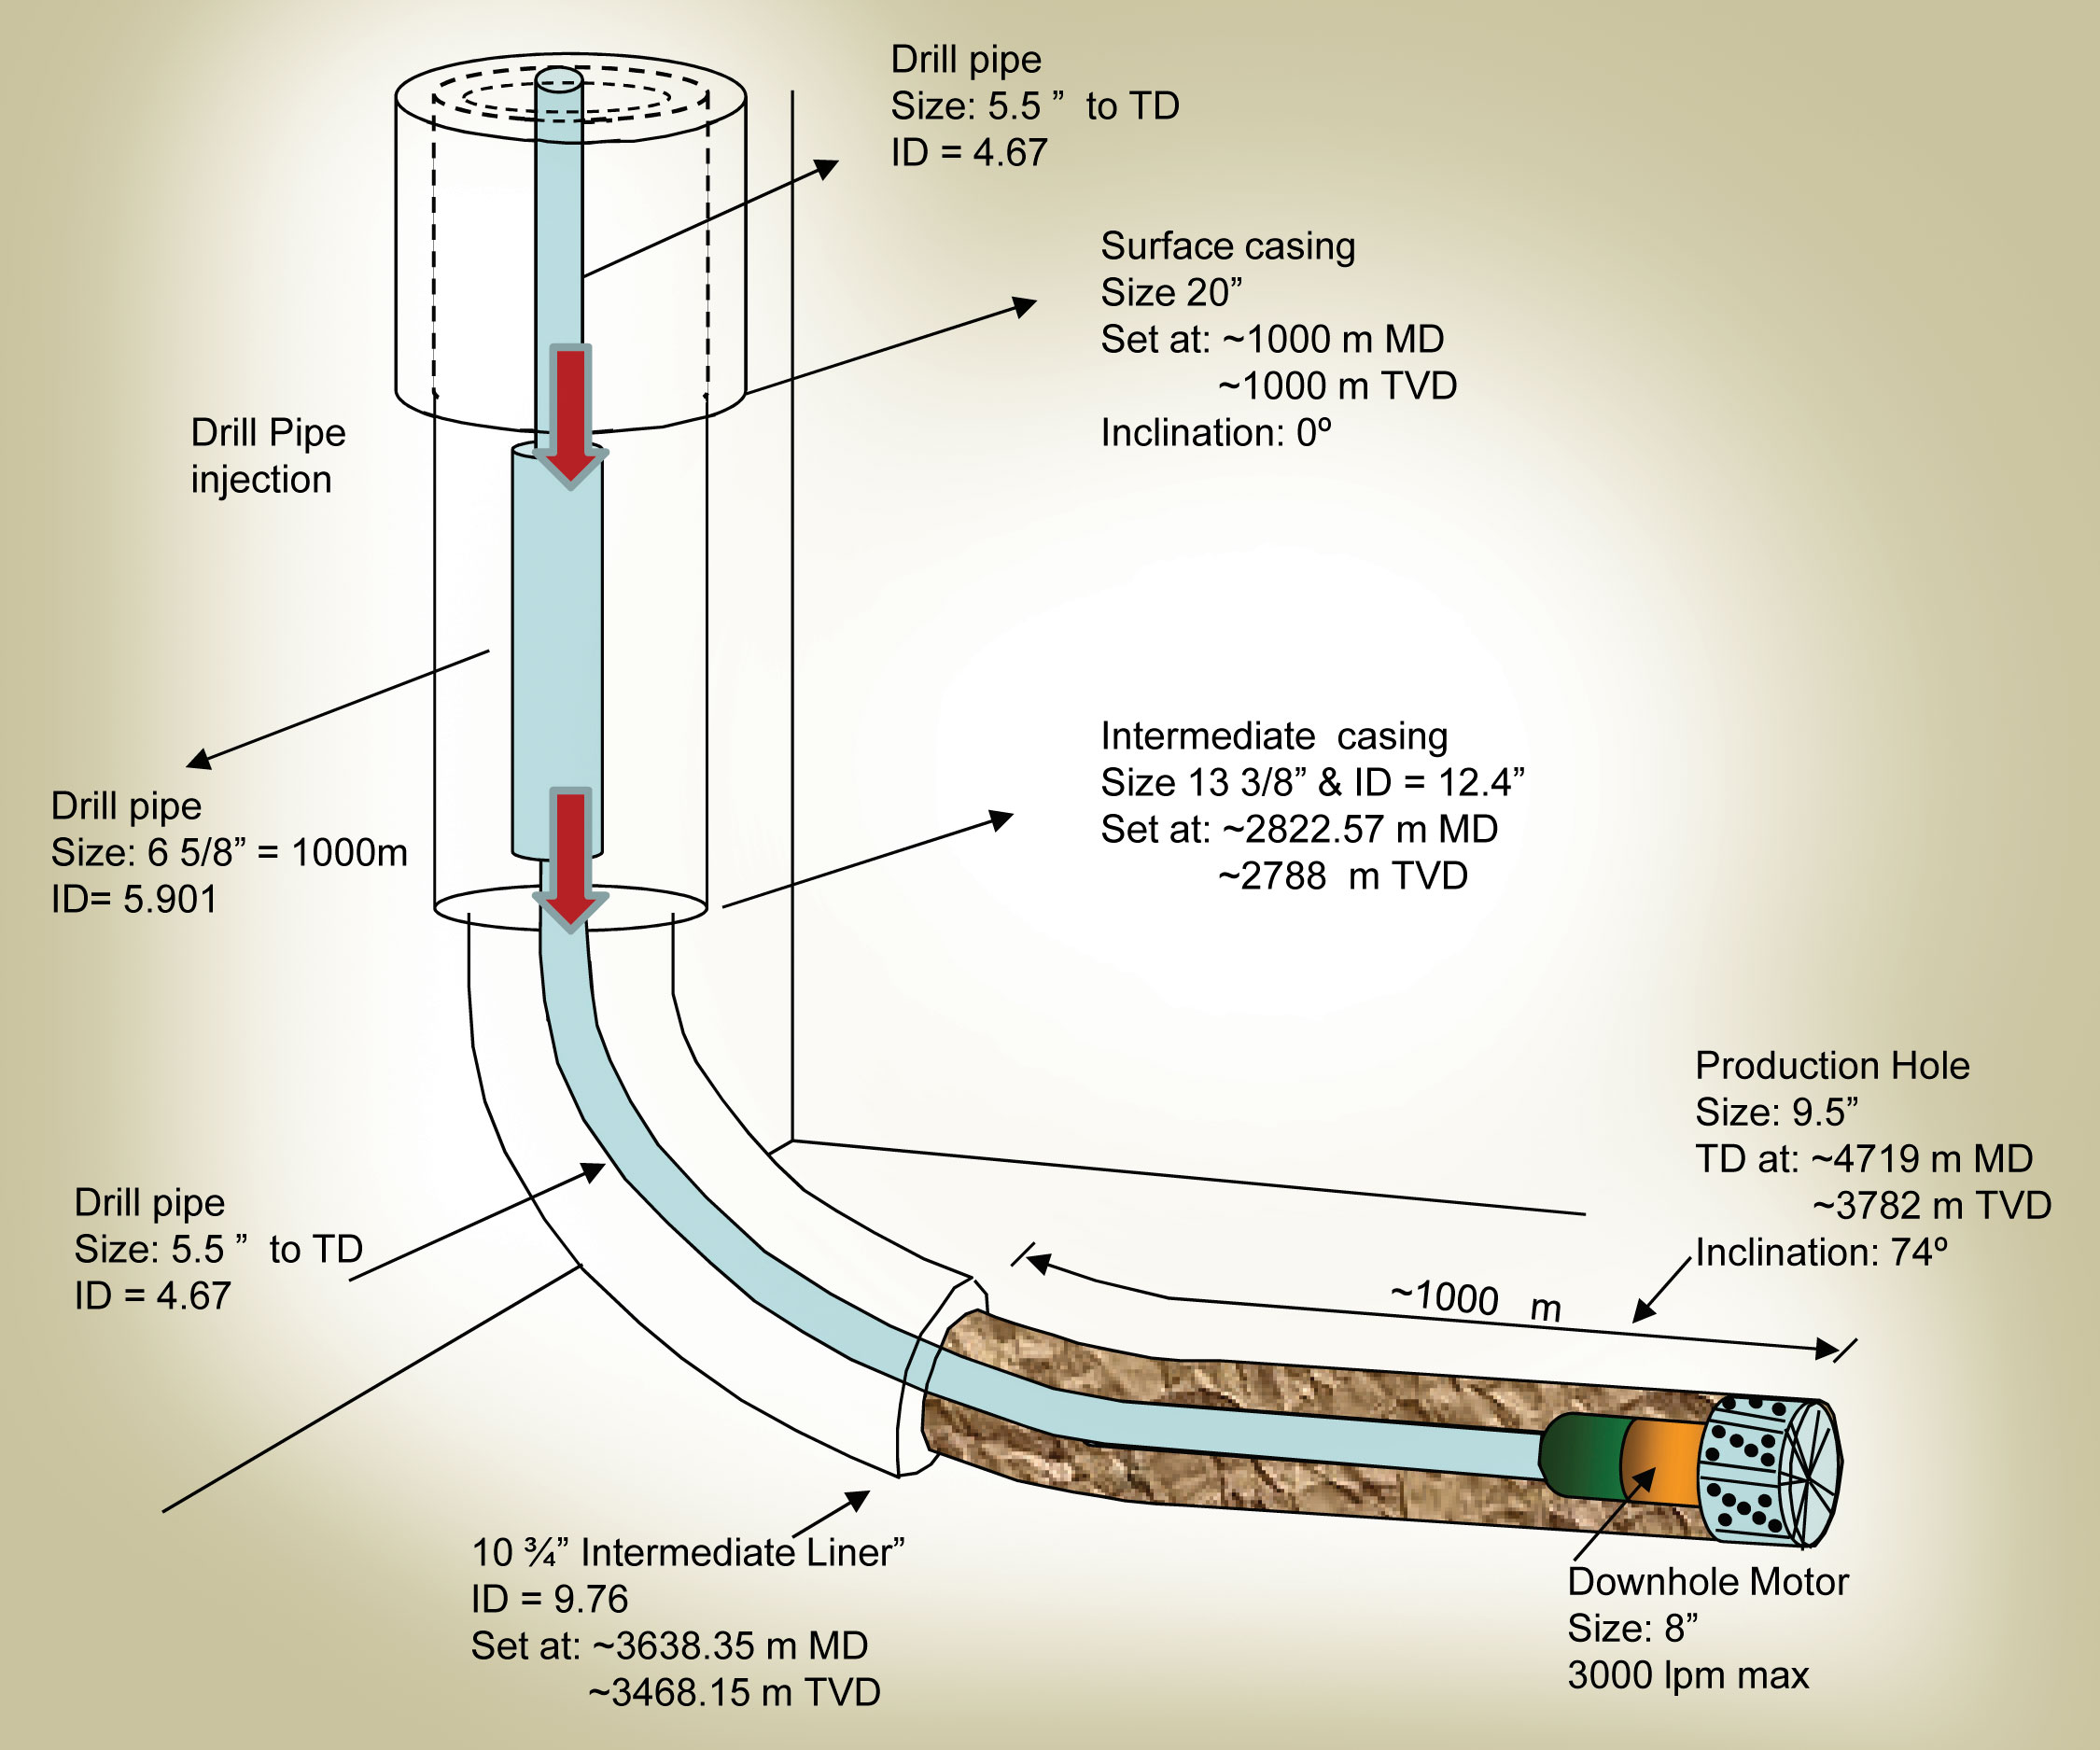
\includegraphics[width=0.55\columnwidth,clip]{./Pics/web_Drillpipe_injection_well_profile-copy.jpg}
          }
       }
    \end{column}
  \end{columns}
\end{frame}
 
 

%%%
%%% Slide
%%%
\begin{frame}
 \frametitle{Phases for Geothermal Project Developments} 
    \begin{enumerate}[1.]
       \item <1-> Preliminary Survey;
       \item <1-> Exploration; 
       \item <1-> Test Drilling;
       \item <2-> \blue{Project Review and Planning};
       \item <1-> Field Development; 
       \item <1-> Power Plant Construction;
       \item <1-> Commissioning and Operation;
    \end{enumerate}
\end{frame}


%%%
%%% Slide
%%%
\begin{frame}
 \frametitle{Phases for Geothermal Project Developments: \\ 4. Project Review and Planning}
    \begin{enumerate}[{4.}1]\scriptsize
       \item <1-> With all information gathered in the previous phases, the project is reassessed;
       \item <2-> This will enable the developer to:
          \begin{enumerate}[(a)]\scriptsize
             \item<2-> Update the numerical reservoir model;
             \item<2-> (Re)Size the development;
             \item<2-> \blue{Secure power purchase agreement (PPA) to help the financial (including risk analysis) model};
          \end{enumerate}
       \item <3-> The \blue{updated} \underline{numerical reservoir and financial models} will allow the feasibility analysis of:
          \begin{enumerate}[(a)]\scriptsize
             \item<3-> Location and design of drilling pads ;
             \item<3-> Design of development wells;
             \item<3-> Specification of drilling targets for remaining production and reinjection wells;
             \item<3-> Forecasts of performance based on simulated reservoir models (including uncertainty quantification);
             \item<3-> Power plant design;
             \item<3-> Transmission access plan;
             \item<3-> Construction budget and costs;
             \item<3-> Terms of the PPA, \blue{budget and revenue projections.}
          \end{enumerate}
    \end{enumerate}
\end{frame}
 


%%%
%%% Slide
%%%
\begin{frame}
 \frametitle{Phases for Geothermal Project Developments} 
    \begin{enumerate}[1.]
       \item <1-> Preliminary Survey;
       \item <1-> Exploration; 
       \item <1-> Test Drilling;
       \item <1-> Project Review and Planning;
       \item <2-> \blue{Field Development}; 
       \item <1-> Power Plant Construction;
       \item <1-> Commissioning and Operation;
    \end{enumerate}
\end{frame}


%%%
%%% Slide
%%%
\begin{frame}
 \frametitle{Phases for Geothermal Project Developments: \\ 5. Field Development }
    \begin{enumerate}[{5.}1]%\scriptsize
       \item <1-> Drilling of a prescribed number of test, production and (re-)injection wells;
       \item <2-> During the drilling, more data is obtained and the model and planning are updated to take into account new data (e.g., better measurement of permeability, porosity, salinity, pH, etc);
       \item <3-> \underline{For an average well of 2 km depth, a drilling time of 40 to 50 days} \underline{(24 hour operation)} is often required;
       \item <4-> In order to \blue{reduce the risk of depletion}, re-injection wells are required to return the geothermal fluids to the reservoir; 
       \item <5-> The \blue{ratio of reinjection} to production wells ranges from as low as 1:4 in high enthalpy resources to as high as 1:1 in lower enthalpy resources; 
       \item <6-> The enthalpy associated with the geothermal fluids, fluid-steam ratio and the power plant technology will also \blue{determine the number of required wells};
       \item <7-> Another key issues are \blue{location and depths of reinjection wells} -- the decision is based on both drilling experience and numerical simulations.
    \end{enumerate}
\end{frame}
 


%%%
%%% Slide
%%%
\begin{frame}
 \frametitle{Phases for Geothermal Project Developments} 
    \begin{enumerate}[1.]
       \item <1-> Preliminary Survey;
       \item <1-> Exploration; 
       \item <1-> Test Drilling;
       \item <1-> Project Review and Planning;
       \item <1-> Field Development; 
       \item <2-> \blue{Power Plant Construction};
       \item <2-> \blue{Commissioning and Operation};
    \end{enumerate}
\end{frame}


%%%
%%% Slide
%%%
\begin{frame}
 \frametitle{Phases for Geothermal Project Developments: \\ 6. Power Plant Construction \\ 7. Commissioning and Operation }
    \begin{enumerate}[1]\setcounter{enumi}{5}
       \item <1-> Power Plant Construction
         \begin{enumerate}[{6.}1]
           \item<1-> Completion of the steam gathering system, coordinated with infrastructure work;
           \item<1-> Power plant construction and well testing.
         \end{enumerate}
       \item <2-> Commissioning and Operation
         \begin{enumerate}[{7.}1]
           \item<2-> Optimisation of the production and injection procedures to enable the most efficient energy recovery and utilisation;
           \item<2-> This will enable the minimisation of operational costs, maximisation investment returns, and to ensure the reliable delivery of geothermal power.
         \end{enumerate}
    \end{enumerate}
\end{frame}
 


























%%%           %%%
%%%  SECTION  %%% 
%%%           %%%
\section{Summary}
%%%
%%% Slide
%%%
\begin{frame}
 \frametitle{Summary}
  \begin{enumerate}
%
     \item <1-> Components 
%
  \end{enumerate}
\end{frame}


\end{document}
